\documentclass{article}
\usepackage{amsfonts, amsmath, amssymb, amsthm, graphicx} % Math 
\graphicspath{ {.././images} }
\usepackage{enumitem}
\setlength{\parindent}{0pt} \oddsidemargin -0.2in \evensidemargin
0.0in \topmargin -1in \textheight 9.9in \textwidth 6.9in

\newtheorem{thm}{Theorem}
\newtheorem{prop}[thm]{Proposition}
\newtheorem{cor}[thm]{Corollary}
\newtheorem{claim}[thm]{Claim}

\newenvironment{problem}[2][Question]{\begin{trivlist}
\item[\hskip \labelsep {\bfseries #1}\hskip \labelsep {\bfseries #2.}]}{\end{trivlist}}

% main content
\begin{document} 

\textbf{Math 158 HW2}

% Q2.5.2
\begin{problem}{2.5.2}
    A tournament is an orientation of a complete graph. Prove that every tournament contains a directed path containing all of its vertices.
\end{problem}
\begin{proof}
    Let $T_n$ be a $n$-vertex tournament. We will prove by induction on $n$ to show that $T_n$ is traceable for all $n$. $T_1$ is obviously traceable as it only contains one vertex. $T_2$ is traceable, as it contains only one directed edge that connects all the vertices in the graph. Suppose that a $T_k$ contains a directed hamiltonian $uv$-path $P$, for some $k \geq 2$. We denote the vertex after $x$ in $P$ as $x^+$, for some $x \in V(P)$. By adding a vertex $w$ and $k$ directed edges to $T_k$, we get a $T_{k+1}$. If $e = (w, u)$ or $(v, w) \in E(T_{k+1})$, we can connect $e$ with $P$ to obtain a hamiltonian path in $T_{k+1}$. If $(w, u), (v, w) \notin E(T_{k+1})$, we know $(u, w), (w, v) \in E(T_{k+1})$ because $N_{T_{k+1}}(w) = V(P)$, which ensures $d_{T_{k+1}}^+(w), d_{T_{k+1}}^-(w) \geq 1$. Hence, there exist $x \in V(P)$ such that $(x, w), (w, x^+) \in E(T_{k+1})$. We can then add $w$ and $(x, w), (w, x^+)$ to $P - (w, w^+)$ to get a directed hamiltonian path in $T_{k+1}$. Thus, if $T_k$ is traceable, then $T_{k+1}$ is also traceable. Therefore, all tournaments are traceable.
\end{proof}

\newpage

% Q2.5.9
\begin{problem}{2.5.9}
    The closure of an $n$-vertex graph $G$, denoted $C(G)$, consists in adding edges between any two non-adjacent vertices $u$ and $v$ such that $d_G(u)+d_G(v) \geq n$. Prove that a graph $G$ is hamiltonian if and only if $C(G)$ is hamiltonian.
\end{problem}
\begin{proof}
    If $G$ is hamiltonian, $G$ contains a hamiltonian cycle $H \subseteq G$. Since $C(G)$ contains $G$ and $V(C(G)) = V(G)$, we have $H \subseteq G \subseteq C(G)$, and thus $C(G)$ is hamiltonian. 
    
    Suppose that $C(G)$ has a hamiltonian cycle $F$. If $F$ does not contain any edges that are not in $G$, then $G$ is hamiltonian. Otherwise, there exists $\{u, v\} \in E(F)$ such that $\{u, v\} \notin E(G)$, which implies $d_G(u)+d_G(v) \geq n$. Let $P = F - \{u, v\}$ be a hamiltonian $uv$-path of $C(G)$, say $v_1v_2\dots v_n$, and $N(v)^+ = \{v_{i+1} : v_i \in N_G(v)\}$. We then have $N(v)^+ \cup N(u) \subseteq V(P)\backslash \{u\}$, which shows that $|N(v)^+ \cup N(u)| \leq n - 1$. Since $|N(v)^+| + |N(u)| = d_G(u)+d_G(v) \geq n$, we have
    \begin{align}
        |N(v)^+ \cap N(u)|
        &= |N(v)^+| + |N(u)| - |N(v)^+ \cup N(u)| \\
        &\geq n - (n - 1) = 1.
    \end{align}
    Hence, $N(v)^+ \cap N(u) \neq \emptyset$. Let $v_k \in N(v)^+ \cap N(u)$, we can then get a new hamiltonian cycle $P - \{v_k, v_{k+1}\} + \{u, v_{k+1}\} + \{v_k, v\}$. This shows that all $e \in E(F)\backslash E(G)$ can be removed from $F$ to obtain a hamiltonian cycle that only consists of edges in $G$, which shows that $G$ is hamiltonian. Therefore, $C(G)$ is hamiltonian if and only if $G$ is hamiltonian.
\end{proof}

\newpage

%2.5.11
\begin{problem}{2.5.11}
    Let $G$ be a hamiltonian bipartite graph of a minimum degree of at least three. Prove that $G$ contains at least two hamiltonian cycles.
\end{problem}
\begin{proof}
    Let $C$ be a hamiltonian cycle in bipartite graph $G(A,B)$, and let $u, v, w \in A$ such that $N_C(u) = \{v, w\}$. Consider the hamiltonian $uv$-path $P = C - \{u, v\}$. Since $G$ is bipartite and $v \in B$, we know $N(v)^+ \in B$, and thus the vertices of $P$ obtained by all possible rotations are all in $B$. Let $G'(A', B') \subseteq G$ such that $C \subseteq G'$ and $d_{G'}(b) = 3$ for all $b \in B'$. We know $G'$ exists because $\delta(G) \geq 3$. Let $H$ be a graph whose vertices are hamiltonian paths of $G'$ starting with the edge $\{u, w\}$, where two hamiltonian paths in $G'$ form an edge of $H$ if they are obtained from one another by rotation. If $Q \in H$ is a hamiltonian path that ends at a vertex $x$, then $Q$ has $3 - 1 = 2$ possible rotations in $G'$ unless $\{u, x\} \in E(G')$, in which case would have $3 - 2 = 1$ rotations instead. In the latter case, $Q$ together with $\{u, w\}$ would form a hamiltonian cycle in $G'$. By the Handshake Theorem, since the number of vertices with odd degrees is even, there is an even number of paths $Q$ in $G'$ which ends at a neighbor of $u$. Therefore, $G'$ has an even amount of hamiltonian cycles. Since $G'$ already contains a hamiltonian cycle $C$, it must contain some other hamiltonian cycle $C'$. Since $C, C' \subseteq G' \subseteq G$, $G$ has at least two hamiltonian cycles.
\end{proof}

\newpage

% 3.8.2
\begin{problem}{3.8.2}
    A tiling of an $m \times n$ chess board is a set of dominoes that cover all the squares on the chess board exactly once (each domino covers two adjacent squares).
\end{problem}
\begin{enumerate}[label=(\alph*)]
    \item For which $m \geq 1$ and $n \geq 1$ does an $m \times n$ chess board having a tiling?
    \begin{proof}[Solution]
        Since the number of squares on the chess board must be even to have a perfect matching, $m$ or $n$ is even. Assume, without loss of generality, that $m$ is even. We will prove by induction on $m$. If $m = 2$,  then we can match each square in one column to one in the adjacent column that is adjacent to it, and this is a perfect matching $M_2$. Suppose that there is a perfect matching $M_k$ for each $k \times n$ chessboard, where $2 \leq k \leq m$ and is even. We can then split a $(m + 2) \times n$ chessboard into a $2 \times n$ and $m \times n$ board. We can then find a perfect matching $M_2 \cup M_m$. This also shows true for even $n$. Therefore, for all $(m,n) \in \{(a, b) \in \mathbb{N}^2: ab \text{ is even}\}$, an $m \times n$ chessboard has tiling. 
    \end{proof}
    
    \item If we remove two squares from an $m \times n$ chessboard, when do the remaining squares have a tiling?
    \begin{proof}[Solution]
        There must be an even amount of squares to have tiling, so if a $m \times n$ chessboard has tiling after two squares removed, then the $m \times n$ chessboard also has an even amount of squares. Thus, $m$ or $n$ needs to be even.

        Assume, without loss of generality, that $m$ is even. Let $G$ be a grid graph whose vertex set contains all squares on a $m \times n$ chessboard, and each pair of vertices forms an edge if they are adjacent to each other on the board. Since $m$ is even, $G$ has a perfect matching. Let $v_{xy}$ correspond to the square in the $x$th row and $y$th column, for some $1 \leq x \leq n$, $1 \leq y \leq m$. Let $\{c_1, c_2\}$ be a set of two colors. We color $v_{xy}$ with $c_1$ if $x + y$ is even and $c_2$ if $x + y$ is odd. This shows that every square can be colored with no same-colored squares being adjacent. Since each domino covers a $c_1$ square and a $c_2$ square, each color must have the same number of squares to have tiling. Therefore, if we remove two squares with the same color, then $G$ does not have a tiling.
        
        Suppose that we remove two squares $u, v$ with different colors. If $n = 1$, then $G - \{u\} - \{v\}$ has a tiling if there are only even components.
        \begin{claim}
            If $m = 2$, then $G - \{u\} - \{v\}$ has a tiling.
        \end{claim}
            Suppose that $u, v$ are each in the first and last rows and $n$ is some natural number. Consider the case where $n$ is odd. Since $u, v$ have different colors, $u, v$ are in different columns. This means that the two columns in $G - \{u\} - \{v\}$ both have $n - 1$ number of squares, which is even. Consider the case where $n$ is even. Since $u, v$ has different colors, $u, v$ are in the same column. This means that the two columns in $G - \{u\} - \{v\}$ have $n$ and $n - 2$ numbers of squares respectively, which are also even. Thus, in both cases, we can tile along the columns and cover all squares, which is a tiling. Suppose that $u, v$ are in the $i$th and $j$th rows, for some $1 < i \leq j < n$. We can then remove the first $i - 1$ rows and the last $n - j$ rows, as there are two columns so we can find a tiling of them by putting a domino in each row. What is left is a $2 \times (j - i + 1)$ board with two corners on both sides removed, which we just proved to have tiling in the first case. Therefore, $G - \{u\} - \{v\}$ has a tiling if $m = 2$.
            
            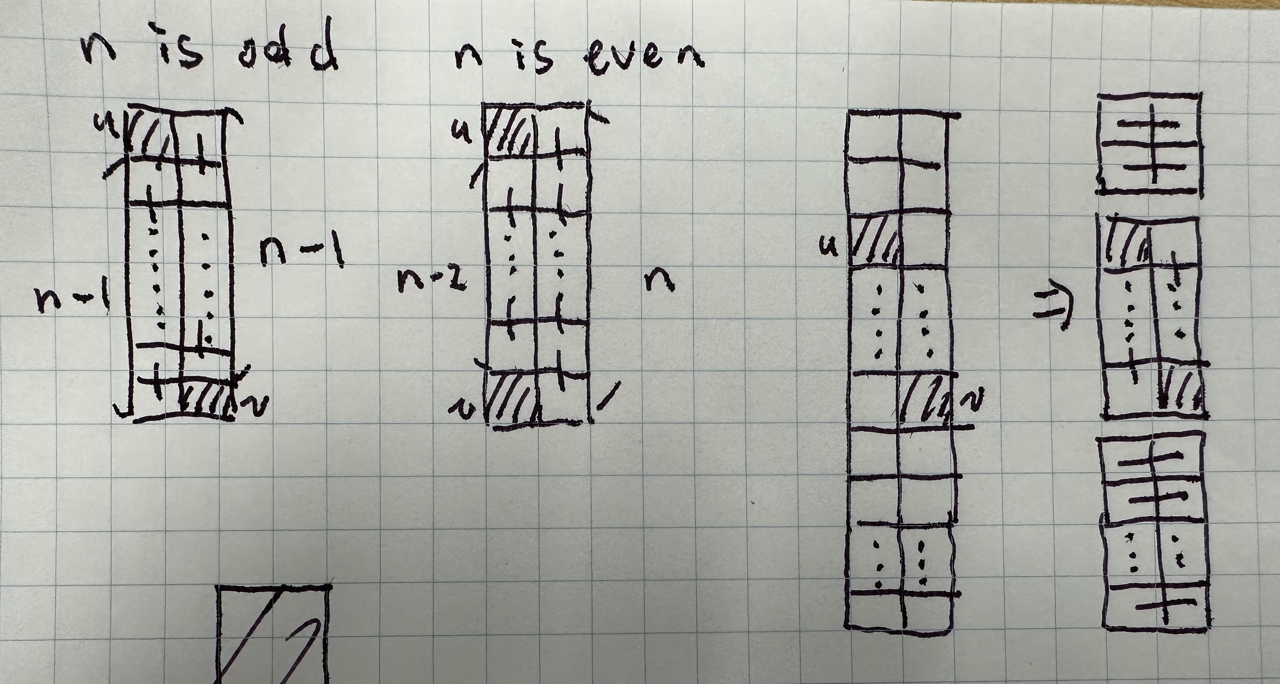
\includegraphics[width=\textwidth]{Q382b1}
        \begin{claim}
            Suppose that $n \geq 2$. If $u, v$ are each in a $2 \times 2$ corner on the opposite side, then $G - \{u\} - \{v\}$ has a perfect matching.
        \end{claim}
        Assume, without loss of generality, that $u$ is in the top left $2 \times 2$ corner and $v$ is in the bottom right $2 \times 2$ corner. Since the $(m - 2) \times (n - 2)$ squares on the bottom left have a perfect matching $M_1$, as it has an even side, we can first take it out. What is left are the first two rows and last two columns of $G$, so we can split it into two parts, a $(m - 2) \times 2$ board $A$ that contains $u$ and a $(2 \times n)$ board $B$ that contains $v$. Let $w \in V(B) \cap N_G(V(A))$ such that $w$ shares the same color with $u$. We remove $w$ from $B$ to $A$, and we then have two parts, $A + \{w\}$ and $B - \{w\}$. We can view $A + \{w\}$ as a $2 \times (m - 1)$ board missing two different color squares $u$ and a square next to $w$. By Claim 1, since both $A + \{w\}$ and $B - \{w\}$ have exactly two columns and are missing two different-colored squares, $A + \{w\}$ and $B - \{w\}$ each has a perfect matching $M_2$ and $M_3$ respectively. Therefore, $G - \{u\} - \{v\}$ has a perfect matching $M_1 \cup M_2 \cup M_3$.

        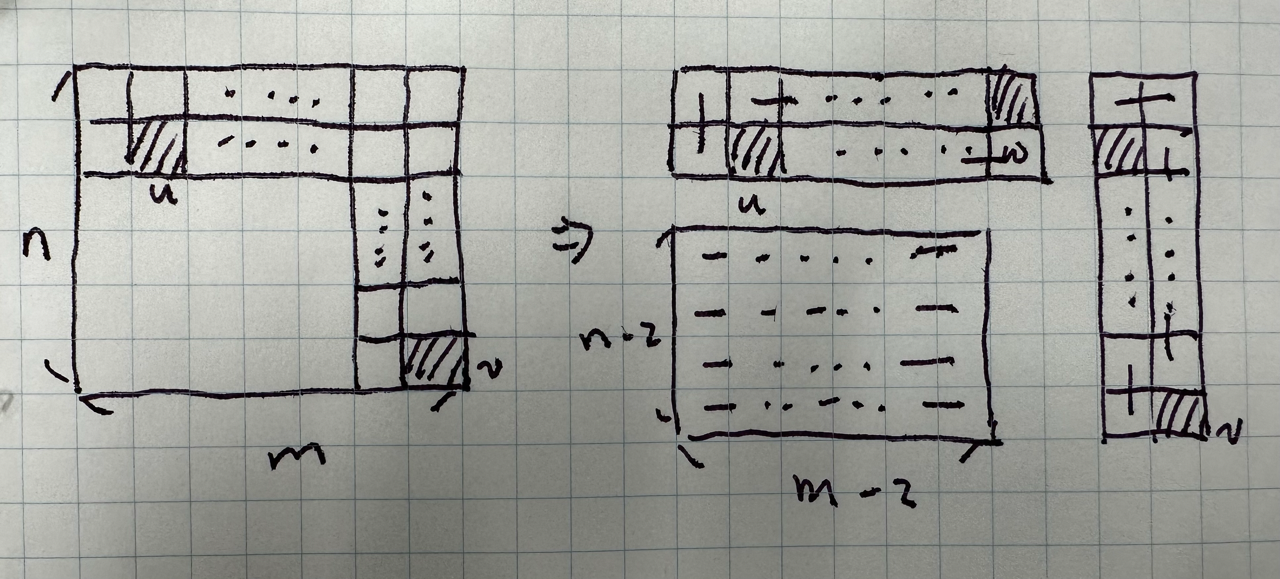
\includegraphics[width=\textwidth]{Q382b2}

        Finally, we will show that $G - \{u\} - \{v\}$ has a perfect matching for all $m, n \geq 2$, $m$ is even. Suppose that $u$ is in the $i$th row $j$th column and $v$ is in the $k$th row $l$th column of $G$. Assume, without loss of generality, that $k \geq i$ and $l \geq j$. We can first take out a $m \times (i - 1)$ board $I$ that contains the first $(i - 1)$ rows of $G$ and a $m \times (n - k)$ board $K$ that contains the last $(n - k)$ rows of $G$. Since they both have an even side $m$, they have a perfect matching $M_i$ and $M_k$ respectively. What's left is a $m \times (k - i + 1)$ board $G'$. We can then take out the left-most $2\alpha$ and right-most $2\beta$ columns of $G'$, where $\alpha$ is the greatest integer such that $2\alpha < j$ and $\beta$ is the greatest integer such that $m - 2\beta > l$ and obtain a $2\alpha \times (k - i + 1)$ board $J$ and a $2\beta \times (k - i + 1)$ board $L$. Since $J$ and $L$ each have an even side $2\alpha$ and $2\beta$, they have perfect matching $M_J$ and $M_L$ respectively. What is left is a $(m - 2(\alpha + \beta)) \times (k - i + 1)$ board $C$ with $u, v$ in opposite side $2 \times 2$ corners. By Claim 2, $C$ contains a perfect matching $M_C$. We now found a perfect matching $M_I \cup M_J \cup M_K \cup M_L \cup M_C$ of $G - \{u\} - \{v\}$. Therefore, if we remove two squares from a $m \times n$ chessboard, it has tiling if and only if $mn$ is even and the two removed squares have different colors and all boards have an even number of squares.
        
        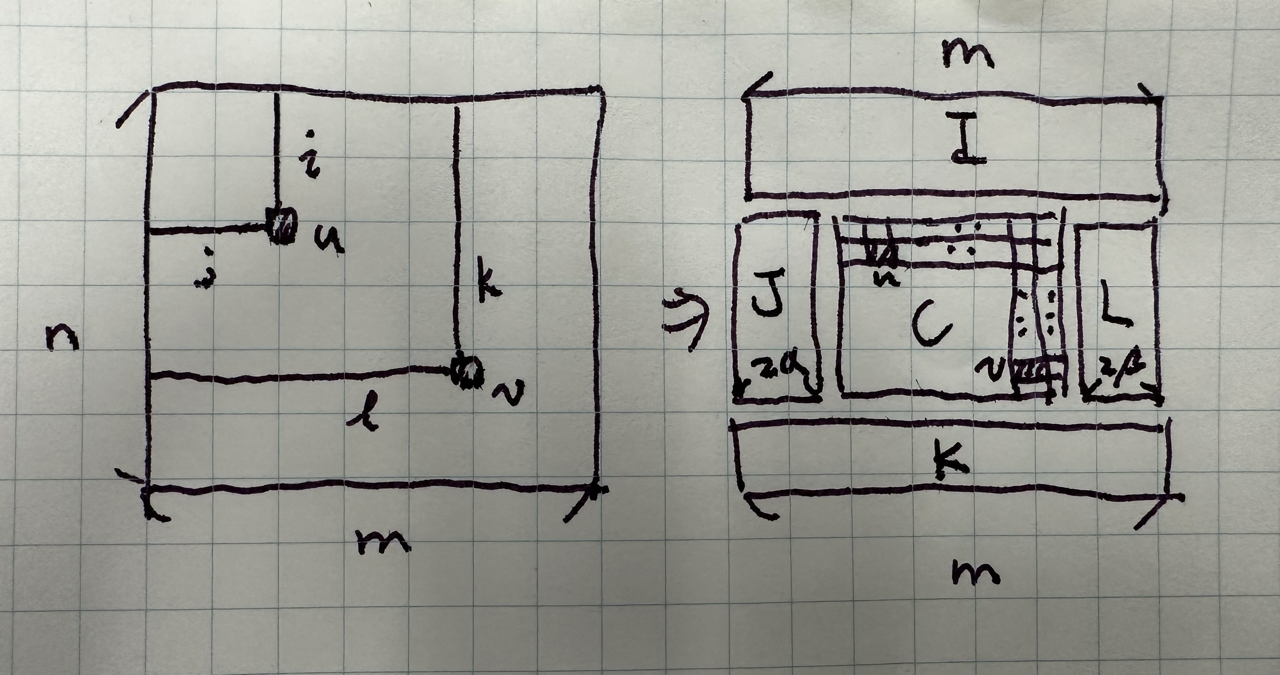
\includegraphics[width=\textwidth]{Q382b3}
    \end{proof}
\end{enumerate}

\newpage

% 3.8.8
\begin{problem}{3.8.8}
    
\end{problem}
\begin{enumerate}[label=(\alph*)]
    \item Let $G$ be an $n$ by $n$ bipartite graph of minimum degree more than $n/2$. Prove that $G$ has a perfect matching.
    \begin{proof}[Solution]
        Suppose that there is a non-hamiltonian $n$ by $n$ bipartite graph of minimum degree at least $n /2$. Amongst all such graphs, let $H(A, B)$ be one with parts $A$ and $B$ and a maximum number of edges. If we add an edge $e = \{v_1, v_{2n}\}$ between non-adjacent vertices in $H$, we would have a graph with a hamiltonian cycle $C$, and so $C - e$ is a hamiltonian path in $H$, say $v_1v_2 \dots v_{2n}$. Assume, without loss of generality, that $v_1 \in A$ and $v_{2n} \in B$. Let $N(v_1)^+ = \{v_{i+1} : v_i \in N(v_1)\}$. Since $N(v_1)^+ \cup N(v_{2n}) \subseteq A$, we have $|N(v_1)^+ \cup N(v_{2n})| \leq n$. Since $\delta(H) > n/2$, we have $|N(v_1)^+| + |N(v_{2n})| \geq n + 1$. Thus, we have
        \begin{align}
            |N(v_1)^+ \cap N(v_{2n})| 
            &= |N(v_1)^+| + |N(v_{2n})| - |N(v_1)^+ \cup N(v_{2n})| \\
            &\geq n + 1 - n = 1.
        \end{align}
        This shows that $N(v_1)^+ \cap N(v_{2n}) \neq \emptyset$, which proves that $H$ contains a hamiltonian cycle, a contradiction. Therefore, there exists a hamiltonian path $P$ in $G$ such, say $u_1 u_2 \dots u_{2n}$. Let $f = \{(u_i, u_{i+1}) : i \text{ is even}\}$. We can then find a perfect matching $M = P - f$ of $G$. Hence, $G$ has a perfect matching.
    \end{proof}
    
    \item Let $G$ be a $2n$-vertex graph of minimum degree at least $n$. Prove that $G$ has a perfect matching.

    \begin{proof}[Solution]
        If $n = 1$, $G$ itself is a perfect matching for $G$. Suppose that $n \geq 2$. By Dirac's Theorem, since $\delta(G) \geq |V(G)|/2$, $G$ contains a hamiltonian path $P$, say $v_1v_2 \dots v_{2n}$. Let $e = \{(v_i, v_{i+1}) \in E(P) : i \text{ is even}\}$, then $M = P - e$ is a perfect matching in $G$. Therefore, $G$ has a perfect matching.
    \end{proof}
\end{enumerate}

\end{document}